\documentclass[11pt, oneside]{amsart}   	% use "amsart" instead of "article" for AMSLaTeX format
\usepackage[margin=1in]{geometry}
\usepackage[]{algorithm2e}
\geometry{letterpaper}
\usepackage{graphicx}
\usepackage{parskip}
\usepackage{amsthm, amsmath, amssymb}

\usepackage{listings}
\usepackage{xcolor}

\usepackage[all]{nowidow}

\definecolor{codegreen}{rgb}{0,0.6,0}
\definecolor{codegray}{rgb}{0.5,0.5,0.5}
\definecolor{codepurple}{rgb}{0.58,0,0.82}
\definecolor{backcolour}{rgb}{0.95,0.95,0.92}

\lstdefinestyle{mystyle}{
    backgroundcolor=\color{white},   
    commentstyle=\color{codegreen},
    keywordstyle=\color{blue},
    numberstyle=\tiny\color{codegray},
    stringstyle=\color{codepurple},
    basicstyle=\ttfamily\footnotesize,
    breakatwhitespace=false,         
    breaklines=true,                 
    captionpos=b,                    
    keepspaces=true,                 
    numbers=right,                    
    numbersep=5pt,                  
    showspaces=false,                
    showstringspaces=false,
    showtabs=false,                  
    tabsize=2
}

\lstset{style=mystyle}

\usepackage[final, colorlinks = true, 
            linkcolor = blue, 
            citecolor = black,
            urlcolor = blue]{hyperref} % For hyperlinks in the PDF

\graphicspath{ {images/} }

\usepackage{datetime2} % Uses YEAR-MONTH-DAY format for dates


%SetFonts
\usepackage{fancyhdr} % Headers and footers

\begin{document}

\title{Homework 4} % Article title
\fancyhead[C]{}
\begin{minipage}{0.295\textwidth} % Left side of title section
\raggedright
CS383: Databases\\ % Your lecture or course
\footnotesize % Authors text size
%\hfill\\ % Uncomment if right minipage has more lines
Isabelle Sanford % Your name
\medskip\hrule
\end{minipage}
\begin{minipage}{0.4\textwidth} % Center of title section
\centering 
\large % Title text size
Homework 4\\ % Assignment title and number
\normalsize % Subtitle text size
Sanderson Elimination Data Stuff \\ % Assignment subtitle
\end{minipage}
\begin{minipage}{0.295\textwidth} % Right side of title section
\raggedleft
\today \\
\footnotesize % Email text size
%\hfill\\ % Uncomment if left minipage has more lines
isanford@brynmawr.edu% Your email
\medskip\hrule
\end{minipage}\\

\section{Database Structure}

\subsection{Original}
bloop :)

First, a very brief review of the two original data sets I'm pulling from:


\subsubsection{Games}
Each row on the Games table represents a single game and collected data about it. There are several columns which are aggregated from the original Player Data table, which I've left out, but a couple of them (like the number of players) were worth keeping track of. I'll also note that a few of these columns aren't actually filled out right now (and others are very incomplete), but I'd rather include them in the structure now than try to add them later. 

\begin{table}[h]
    \begin{tabular}{ll}
    \textbf{Column}       & \textbf{Description} \\
    \hline 
    format       & category of game (e.g. LG, meaning Long Game)\\
    number       & nth game in its category   \\
    game string  & format + number (e.g. LG25)   \\
    \# Players   & number of players in the game         \\
    \# Cycles    & number of ``rounds'' the game took        \\
    \# Posts     & total \# of posts in entire game thread          \\
    Fundamentals & basic structure of game (e.g. Faction, V/E)    \\
    Complexity   & complexity of ruleset (e.g. Standard)          \\
    Role madness & whether every player had a role                        \\
    Anon number  & if the game was anonymized, what number was it         \\
    Mechanics    & how broken/balanced the game's mechanics/rules were \\
    Distribution & how broken/balanced the arrangement of roles/teams was \\
    \# Elims     & number of ``eliminators'' (Evil team)                    \\
    \# Survivors & number of players alive at the end of the game         \\
    GM(s)        & person or people who ran the game                      \\
    IM           & forum mod that ``supervised'' the game                   \\
    Title   & Linked title of game thread                            \\
    World        & setting of the game  (e.g. Scadrial, Lord of the Rings)       \\
    start date   & date the first cycle started                           \\
    end date     & date the last cycle ended                                           
    \end{tabular}
    \end{table}


\subsubsection{Player Data}
The Player Data table is the majority of the raw data. It contains one row for every player that interacted with any game: that is, a particular game would have a bunch of rows containing the data for each player in that game, and then additionally rows indicating who ran and supervised that game. This table is currently about 5000 rows. 

\begin{table}[h]
    \begin{tabular}{ll}
    \textbf{Column}       & \textbf{Description} \\                                                          
    \hline
    ID              & number tracking chronological order of entries                         \\
    Player          & name of player                                                         \\
    Alignment       & what team the player was on (e.g. ``E'' for evil)                     \\
    Faction Outcome & whether the player won or lost (e.g. ``W'' for win)                  \\
    First Hit       & cycle in which the player was first attacked                           \\
    Last Hit        & cycle in which the player was last attacked                            \\
    \# of Hits      & number of attacks total which hit the player                           \\
    Death/Survival  & how the player died (or if they survived) (e.g. ``E'' for killed by evil team)   \\
    Inactive        & whether the player went inactive (stopped playing) during the game     \\
    GM(s)           & if player ran game (in which case most of above columns will be empty) \\
    Main?           & whether the player was the main GM or helping out                      \\
    Mod             & whether the player was the forum moderator supervising the game        \\
    Game format     & category of the game (same as in Game table)                           \\
    Game \#         & \# of the game within that category (same as in Game table)            \\
    Game string     & combination of the above 2 (same as in game table)                     \\
    Role            & ability of player during the game, if any                              \\
    Secondary role  & secondary ability of player if present                                           
    \end{tabular}
\end{table}



\subsection{Mongo}

Let's start with Mongo, since the structure of that database is much more similar to the original data. The database contains two collections: \texttt{players} and \texttt{games}, since those are the two major entry points for asking questions about the data. I will admit that I put much less effort into these than the SQL data, partly because I didn't have to worry as much about messy data, but mainly because I like SQL better and plan to use that database past the end of this course. Given more time and interest, these collections would be somewhat more robust. There are also currently a lot of places where a document contains something like \texttt{"mechanics": nan}, which should technically just be left out of the document altogether. 


\subsubsection{games}
The \texttt{games} data is actually fairly close to what the original Games table contained, and looks approximately like this: 

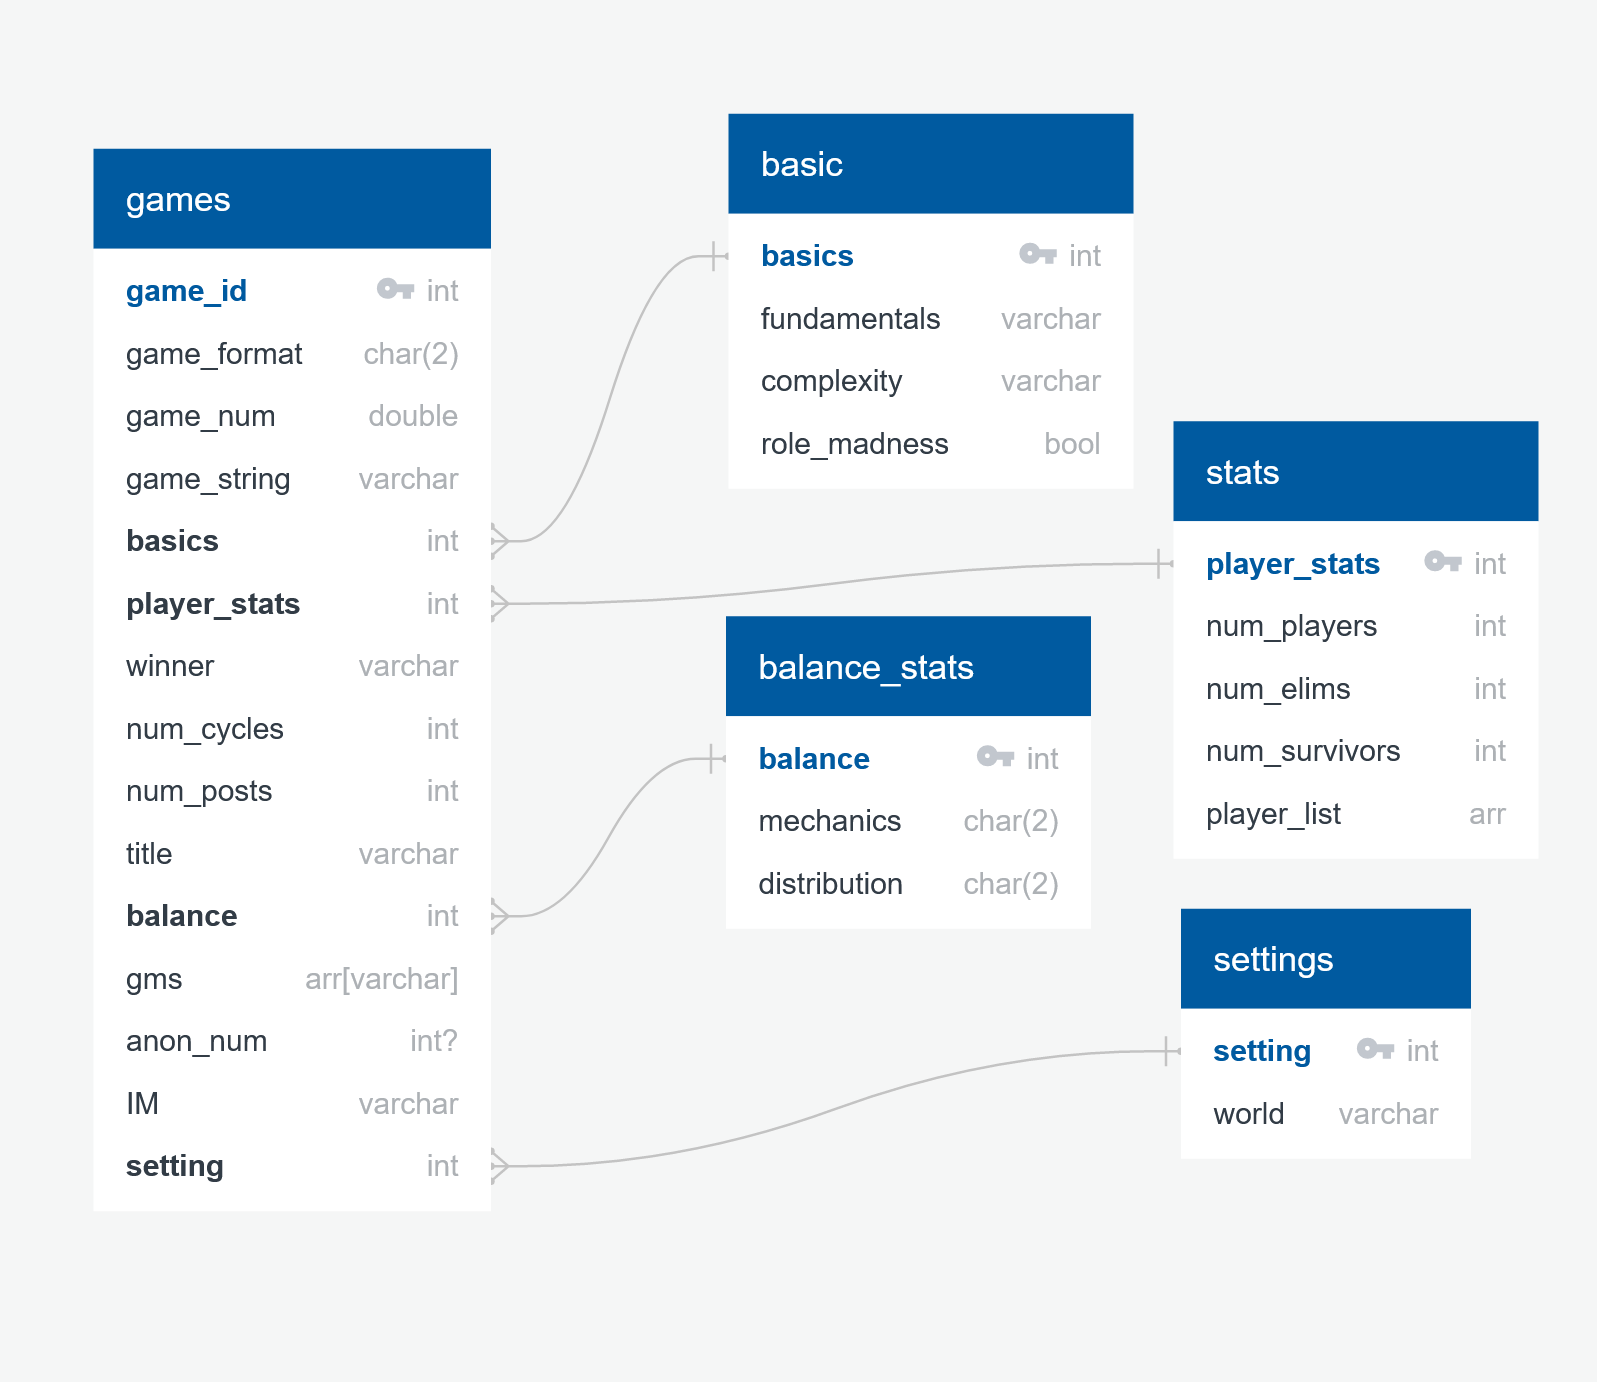
\includegraphics[scale=0.5]{../mongo/mongo_games_v0.png}

I've included an example below (real data, albeit slightly truncated for space), but essentially the Game data is split into sensible categories (similar to those on the actual sheet), and there's a player list pulled from the Player Data. That player list doesn't contain any stats about what happened to the player in that game (although it could, and arguably should), but the name is enough to look up the relevant data from the \texttt{players} collection. I've also kept some of the summary stats (like the number of players) in Mongo, for easy access to especially common ones without having to cross-reference with \texttt{players}.

\begin{verbatim}
{
    'format': 'MR',
    'game_num': 38.1,
    'game_string': 'MR38.1',
    'basics': {
        'fundamentals': 'U', 
        'complexity': 'Basic', 
        'role_madness': False
    },
    'player_stats': {
        'num_players': 18.0,
        'num_elims': 5.0,
        'num_survivors': 15.0,
        'player_list': [
            'Haelbarde',
            'Straw',
            ...
        ]
    },
    'winner': 'E',
    'num_cycles': nan,
    'num_posts': nan,
    'title': 'The Council of Elrond',
    'balance': {
        'mechanics': nan, 
        'distribution': nan
    },
    'setting': {
        'world': 'Lord of the Rings'
    },
    'GMs': ['Elbereth', 'Elbereth'],
    'IM': 'little wilson'
}
\end{verbatim}
And yes, I'm marked as having ran that game twice. No, I don't know why. 

\subsubsection{players}
The \texttt{players} collection, on the other hand, isn't very like the original Player Data. Instead, it's a version of that data aggregated by player, like so:

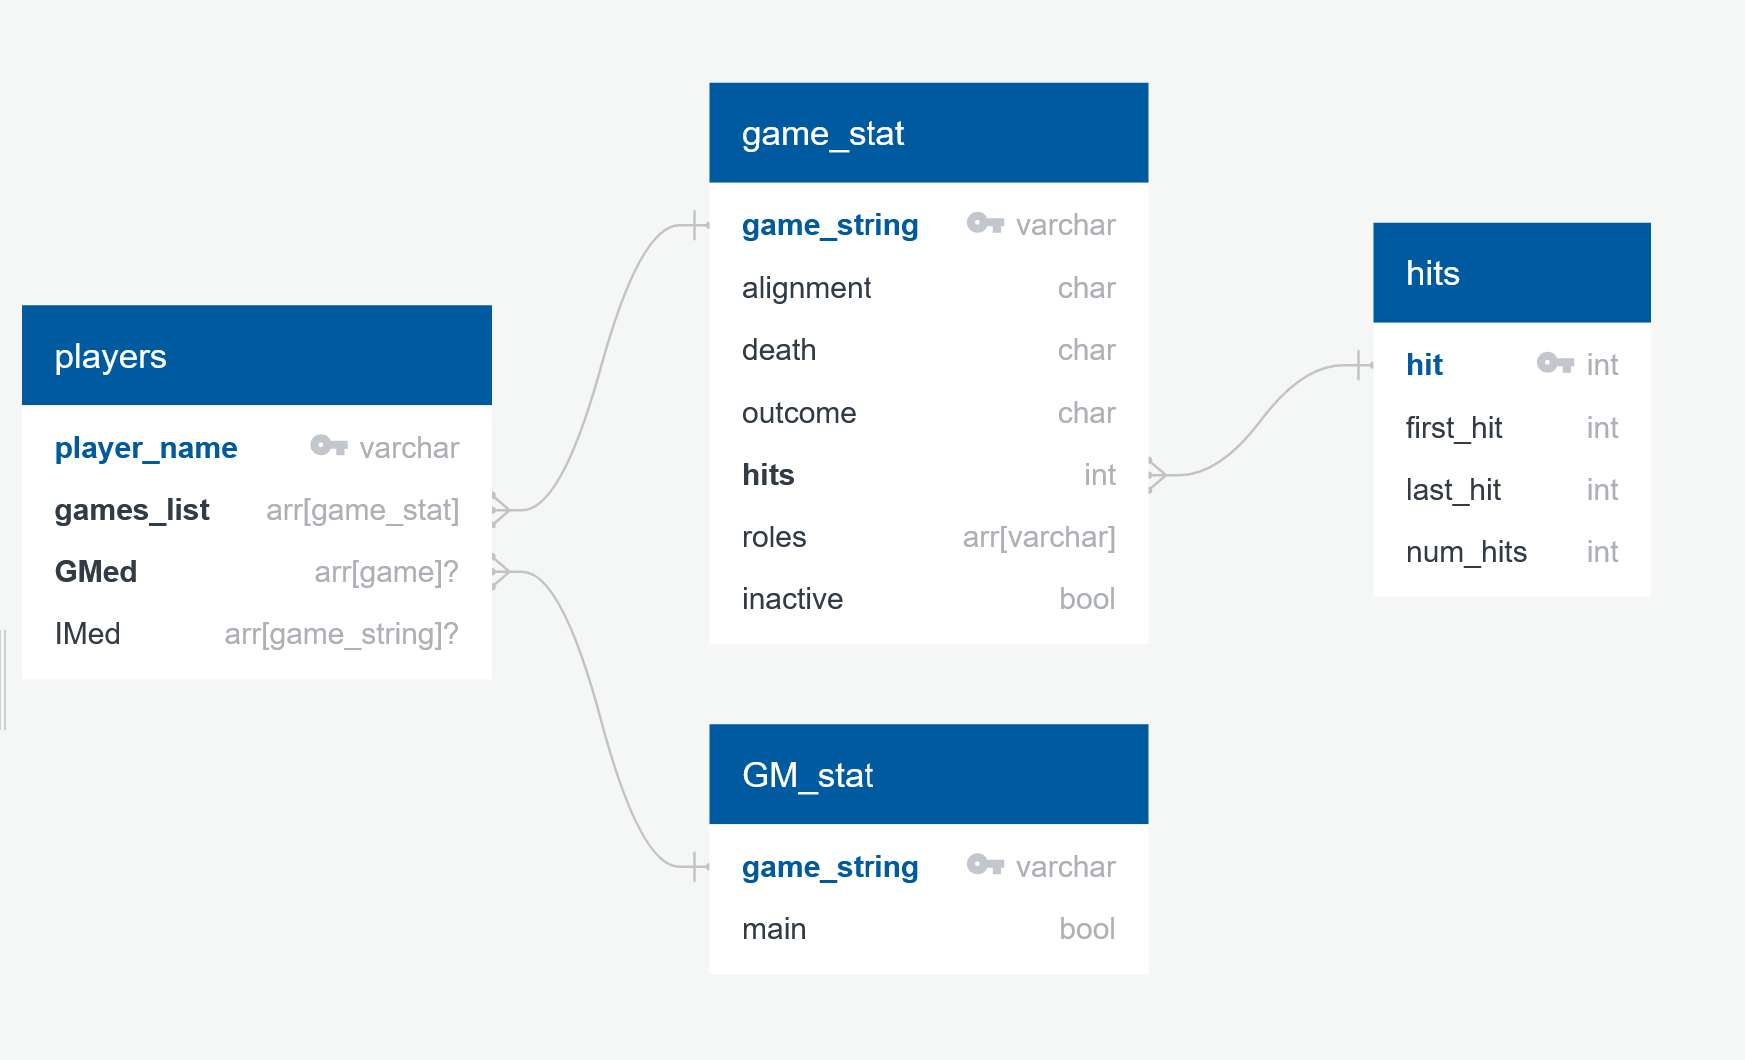
\includegraphics[scale=0.5]{../mongo/mongo_players_v0.png}

Again, I've included an example below, this time of my own document (though again truncated for space). 

\begin{verbatim}
{
    'player_name': 'Elbereth',
    'games': [
        {
            'game_string': 'LG15.2',
            'alignment': 'G',
            'death': 'S',
            'result': 'W',
            'hits': {
                'first': nan, 
                'last': nan, 
                'num': 0.0
            },
            'roles': ['Kill', nan],
            'inactive': False
        },
        ...
    ],
    'GMed': [
        {'game_string': 'QF11', 'main': False},
        {'game_string': 'LG19', 'main': True},
        ...
    ],
    'IMed': [
        {'game_string': 'MR42'},
        {'game_string': 'LG68'},
        {'game_string': 'LG70'},
        ...
    ]
}
\end{verbatim}

Though it was true to an extent in the last collection, it's much more noticeable in this one that you need some outside knowledge to decipher what's going on, particularly in the alignment/death/result values. Those are based on key tables present in the SQL database (and in the original table), but absent here - while having a separate table and just being careful about how you order queries would work and avoid joins, ideally the single characters would just be replaced by a more helpful description, like "Good" / "Survived" / "Won" and so on.

I wasn't sure what to do with the second list, that is `GMed' - the games that you've run. The Player Data sheet only has the two fields shown there easily accessible, and `game\_string' could be used as a key to look up any of the games in the \texttt{games} collection, but it'd still maybe be convenient to have a little more summary information here. (The `GMed' list is probably fine; it's a list only present in the dozen or so people that have been forum moderators over the years, since each game gets supervised by one of them.)


\subsection{SQL}

For putting all this into SQL, I went much more heavy on splitting out things, making key tables, etc, so the final structure looks like this: 

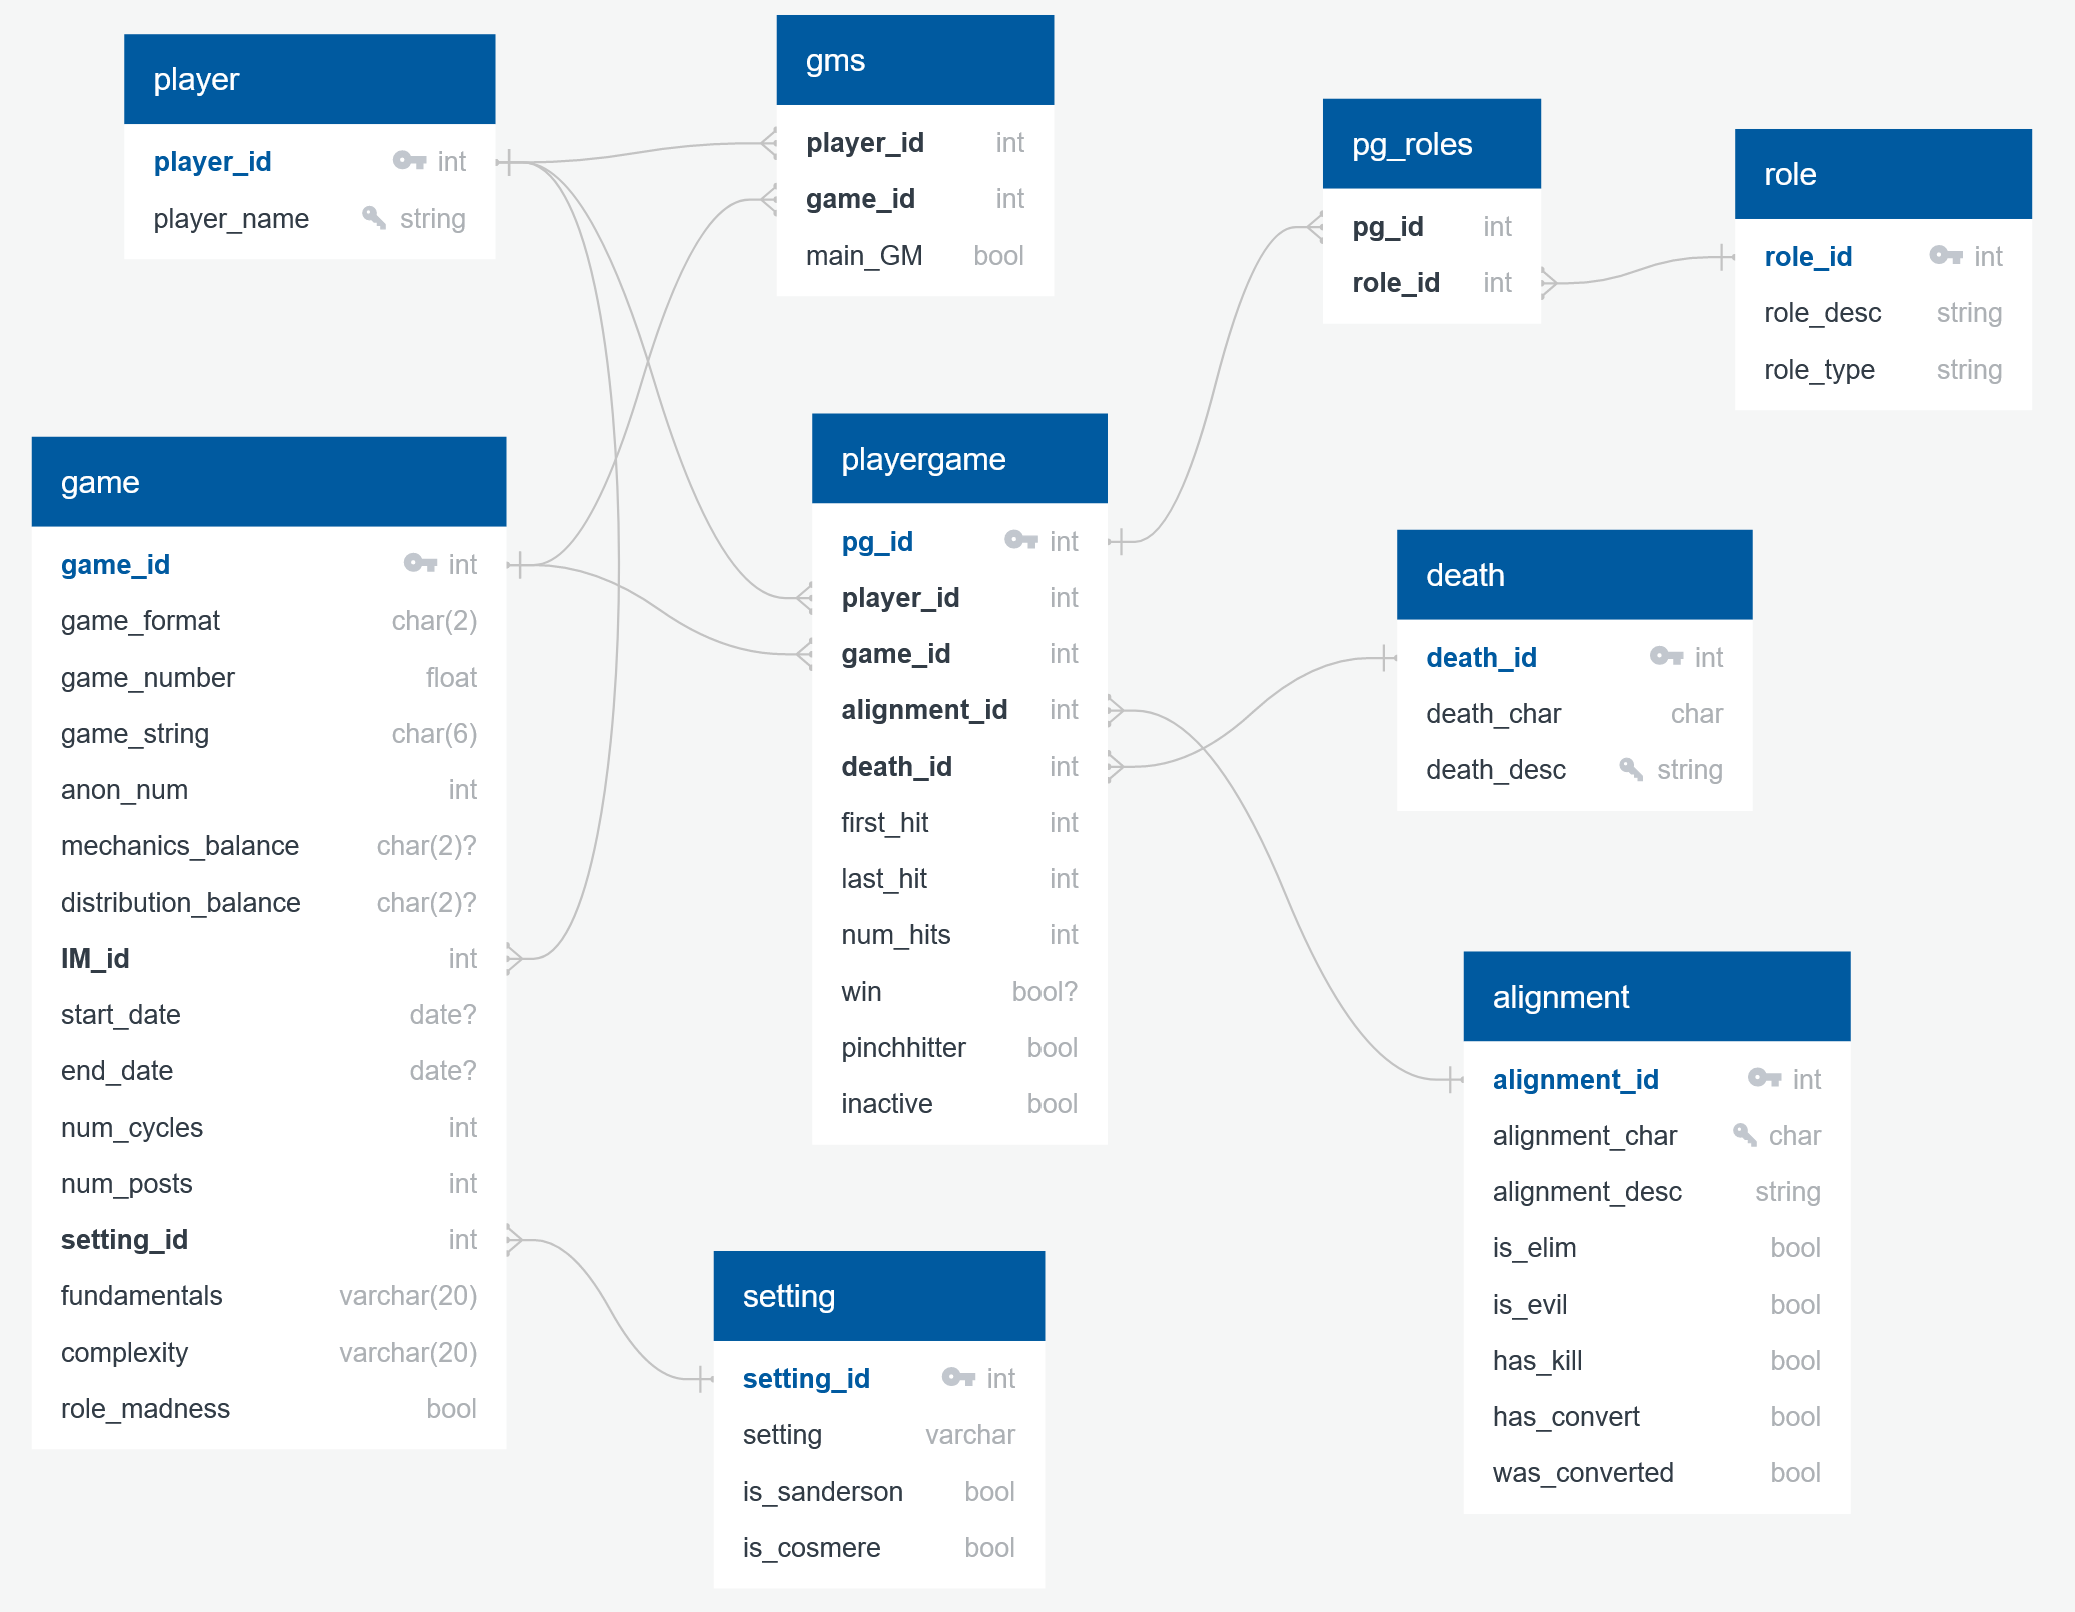
\includegraphics[scale=0.5]{../diagrams/se diagram v3.png}

Each player, game, alignment (team), death type, game setting, and role gets its own integer primary key in separate tables. That's most important for \texttt{player}, as players are both referenced all over the place and may change their name over time. 

The \texttt{game} table looks most like the original data, as most of that table is in fact data that applies only to the game in question or that doesn't need any information attached. (That said, I could have made key tables for the two balance columns, the fundamentals column, and the complexity column. I didn't partly because those would be very small tables, and partly because what those columns actually look like in the spreadsheet is currently in flux anyway.) The only notable key table connection there is to \texttt{setting}, since it's helpful to hold a couple of booleans about each setting in addition to the setting itself for easy querying.

The \texttt{playergame} table contains very similar information to the original Player Data table, and is still a few thousand rows (not the full five thousand since GMs, IMs, etc have been moved to their own spots), but nearly half the columns are integers that connect to varying key tables. Some of these aren't very interesting (the \texttt{death} table doesn't contain any information that wouldn't be as easily gathered by just putting the death description into \texttt{playergame}), but some of them (like \texttt{alignment}) have a bunch of extra data that makes certain queries much easier. (There are seven different types of evil teams represented, each of which has their own id. Having an is\_evil boolean is much, much nicer than having to specify all seven options.)

As I mentioned, the \texttt{gms} table has been separated out. It would be more convenient to just have a row inside \texttt{game}, but the problem is that there can be (and often are) multiple GMs running a single game. So there's a small table with just a player and a game they ran in each row, plus a boolean indicating whether they were the ``main'' GM or not. 

The last branch I haven't described here is the \texttt{pg\_roles} table and its associated \texttt{role} key table. These are the most tentative tables, mainly because we only recently started collecting role data and less than a quarter of the data is filled in right now. But the idea is that a player can (and often does) have multiple roles in a single game, which means putting roles into \texttt{playergame} wouldn't work without duplication somewhere or using arrays. Instead, I gave \texttt{playergame} a primary key ID, and the intention is for \texttt{pg\_roles} to list roles which a certain player in a certain game had. 


\section{Queries}

\subsection{Question:} What games have I ("Elbereth") played? 

SQL answer: 
\begin{lstlisting}[language=SQL]
    with my_games as (
        select game_id from playergame 
        where playergame.player_id IN (
            select player_id from player where player_name LIKE 'Elbereth'
        )
    )
        
    select game_string from game natural join my_games;
\end{lstlisting}
    
% Mongo answer:
% \begin{lstlisting}[language=Javascript]


% \end{lstlisting}

\subsection{Question:} When the evil team wins, what percentage of it (on average) is alive at the end? 

SQL answer:
\begin{lstlisting}[language=SQL]
select
\end{lstlisting}

Mongo answer:


\subsection{Question:} Do games where the evil team wins last longer/shorter than when they don't? (More broadly - does which team won correlate any with game length?)

SQL answer:
\begin{lstlisting}[language=SQL]
-- all factions that won for each game and how many ppl 
WITH by_game AS (
    select game_id, alignment_id, count(player_id) as num_won
    from playergame
    where win
    group by game_id, alignment_id
    order by game_id
),

-- above with cycle length for each game
with_nums AS (
    SELECT * 
    FROM by_game 
        NATURAL JOIN (select game_id, num_cycles from game) AS cycle_nums
), 

-- grouped by alignment
by_alignment AS (
    SELECT alignment_id, avg(num_cycles) as avg_cycle, count(num_cycles) as num_games
    FROM with_nums 
    GROUP BY alignment_id
)

-- adding alignment description
SELECT alignment_desc, avg_cycle, num_games, is_evil 
    FROM by_alignment NATURAL JOIN alignment;
\end{lstlisting}

Mongo answer:


\section{univ}

\begin{lstlisting}[language=SQL]
with course_counts as 
    (select course_id, count(course_id) as count from takes group by course_id),

top_two as (
    select * from course_counts 
    where course_id in 
        (select course_id from course where dept_name like 'Comp. Sci.')
    order by count desc
    limit 2
)

select title, count
    from top_two natural join course 
    order by title;
\end{lstlisting}

Resulting table: 

\begin{lstlisting}[language=SQL]
with thecourse as (select course_id, sec_id, count(sec_id) as c 
    from takes 
    where semester like 'Fall' and year = '2009'
    group by sec_id, course_id
    order by c desc limit 1)

select course_id, sec_id, c, title from thecourse natural join course;
\end{lstlisting}
\textbf{Answer: } Section 1 of course 105 (Image Processing) with 327 students. 

\begin{lstlisting}[language=SQL]

with creds as (select course_id, credits from course),

takes_creds as (select course_id, id, grade, credits 
    from takes natural join creds), 

takes_pts as (select *, credits*points as cp 
    from takes_creds natural join grade_points),

takes_gpa as (select id, 
    sum(credits) as tot, 
    sum(cp) as totgrad, 
    sum(cp)/sum(credits) as gpa 
    from takes_pts 
    group by id
    order by gpa
    limit 3)

select id, name, gpa from student natural join takes_gpa;

\end{lstlisting}


\subsection{3 lowest and 3 highest GPAs}

\begin{lstlisting}[language=SQL]
    with creds as (select course_id, credits from course),

takes_creds as (select course_id, id, grade, credits 
    from takes natural join creds), 

takes_pts as (select *, credits*points as cp 
    from takes_creds natural join grade_points),

takes_gpa as (select id, 
    sum(credits) as tot, 
    sum(cp) as totgrad, 
    sum(cp)/sum(credits) as gpa 
    from takes_pts 
    group by id), 

gpa_low as (select * from takes_gpa order by gpa limit 3), 
gpa_high as (select * from takes_gpa order by gpa desc limit 3), 
gpa as (select * from gpa_low union select * from gpa_high)

select id, name, gpa
    from gpa natural join student
    order by name;
\end{lstlisting}

Table: 

\begin{lstlisting}[language=SQL]
    select id
    from takes 
    group by id
    having min(year) > 2004
    order by id
    limit 5;
\end{lstlisting}
(Note: the limit is greater than 2004 there because using 2005 as the lower limit gave exactly 1 student, and the wording is ambiguous.)


Find the name of the instuructor and salary of the highest paid instructor in all departments whose name starts with A.
\begin{lstlisting}[language=SQL]
    select * from instructor where name like 'A%' order by salary desc limit 1;
\end{lstlisting}

\textbf{Answer: } Arias, \$104,563.38 in Statistics. (The wording here arguably means per department, but the only three instructors whose names start with A are all in statistics as far as I can tell. )

\begin{lstlisting}[language=SQL]
with ret as (select dept_name, max(salary) as m 
    from instructor 
    group by dept_name 
    order by max(salary)
    limit 1)

select name, salary, ret.dept_name 
    from instructor, ret 
    where instructor.dept_name = ret.dept_name 
        and instructor.salary = ret.m;
\end{lstlisting}
\textbf{Answer: } Soisalon-Soininen, Pyschology, \$62,579.61.


\section{rocket}

\begin{lstlisting}[language=SQL]
select apogee, date from launch where apogee > all ( select apogee from launch where date_part('year', date)=1957);

select apogee, date from launch where apogee > ( select max(apogee) from launch where date_part('year', date)=1957);
\end{lstlisting}
            
The former query selects the entire set of 1957 launches, and then compares every row in the table to every single row in that subset (to make sure that the apogee is greater than \textit{all} the 1957 ones). The latter finds the maximum apogee from 1957, and then compares every row in the table to just that single number, which is much faster (roughly by a factor of however many things launched in 1957, though optimization may change that). 


\begin{lstlisting}[language=SQL]
with lat_date as (select hid, min(date) as min
    from observation 
    where hid in 
        (select hid
            from observation natural join hurricane
            where name like 'UNNAMED'
            group by hid
            order by max(date) desc
            limit 5
        )
    group by hid),

all_obvs as (select observation.*
    from observation join lat_date on true 
    where observation.hid = lat_date.hid
    and observation.date = lat_date.min
    ),

min_times as (select hid, min(time) as mintime
    from all_obvs
    group by hid)

select all_obvs.* from min_times join all_obvs on true 
    where all_obvs.hid = min_times.hid and
    all_obvs.time = min_times.mintime;
\end{lstlisting}
(I apologize for how involved this is and it definitely could be better but it works.)


\begin{lstlisting}[language=SQL]
with eastern as (
    select hid, date, time, type, latitude, latitudehemi, 
        maxsustained, longitude * -1 as newlong
    from observation
    where longitudehemi like 'E'),

western as (
    select hid, date, time, type, latitude, latitudehemi, 
        maxsustained, longitude as newlong
    from observation
    where longitudehemi like 'W')
    
(select * from eastern) union (select * from western);
\end{lstlisting}

p
\begin{lstlisting}[language=SQL]
with eastern as (
    select hid, date, time, type, latitude, latitudehemi, 
        maxsustained, longitude * -1 as newlong
    from observation
    where longitudehemi like 'E'),

western as (
    select hid, date, time, type, latitude, latitudehemi, 
        maxsustained, longitude as newlong
    from observation
    where longitudehemi like 'W'),
    
un as (select * from eastern union select * from western)

select date, latitude, newlong, name from un natural join hurricane order by newlong limit 1;
\end{lstlisting}




\end{document}


